%%%%%%%%%%%%%%%%%%%%%%%%%%%%%%%%%%%%%%%%%%%%%%%%%%%%%%%%%%%%%%%%%%%%%%
% Lớp 10 | Mệnh đề. Tập hợp | Các phép toán tập hợp
% Dạng 0D1?3-1: Giao và hợp của hai tập hợp (rời rạc)
% Số câu: 79  (sinh tự động bởi tach_cau.py; từ nay thầy sửa trực tiếp file này)
%%%%%%%%%%%%%%%%%%%%%%%%%%%%%%%%%%%%%%%%%%%%%%%%%%%%%%%%%%%%%%%%%%%%%%

%%%%%%%%%%%%%%%% TRẮC NGHIỆM 4 PHƯƠNG ÁN %%%%%%%%%%%%%%%%

% nguồn: MaHoaNH_TracNghiem_Lop10
\begin{ex}%[0D1N3-1]%[ma:55836a3d]
	Cho tập hợp $X=\{1;5\}$, $Y=\{1;3;5\}$. Tập $X\cap Y$ là tập hợp  nào sau đây?
	\choice 
		 {$\{1\}$}
		 {$\{1;3\}$}
		{$\{1;3;5\}$} 
		{\True  $\{1;5\}$}
	\loigiai{ 
		Ta có $X\cap Y$ là tập  hợp gồm các phần tử vừa thuộc $X$ và vừa thuộc $Y$.
	} 
\end{ex}

% nguồn: MaHoaNH_TracNghiem_Lop10
\begin{ex}%[0D1N3-1]%[ma:1466365c]
	Cho tập hợp $X=\{a;b\}$,  $Y=\{a;b;c\}$. $X\cup Y$ là tập hợp nào sau đây?
	\choice 
		 {$\{a;b;c;d\}$}
		 {$\{a;b\}$}
		{\True $\{c\}$} 
		{$\{a;b;c\}$} 
	 \loigiai{
		Ta có $X\cup Y$ là tập hợp gồm các phần  tử thuộc $X$ hoặc thuộc $Y$.
	} 
\end{ex}

% nguồn: MaHoaNH_TracNghiem_Lop10
\begin{ex}%[0D1N3-1]%[ma:537e4d83]
	Cho tập hợp $H=\{-1;2;x;y\}$, $N=\{x;a;1\}$. $H\cup N$ là tập hợp nào  sau đây?
	\choice 
		{$\{x;1\}$} 
		{$\{-1;2;x;y;a\}$} 
		 {$\{-1;2;y\}$}
		{\True  $\{-1;1;2;x;y;a\}$}
	\loigiai{ 
		Ta có $H\cup  N=\{-1;1;2;x;y;a\}$.
	} 
\end{ex}

% nguồn: MaHoaNH_TracNghiem_Lop10
\begin{ex}%[0D1N3-1]%[ma:d05ebb53]
	Cho hai  tập hợp $A$ và $B$. Tập hợp $A\cup B$ là
	 \choice
		{tập hợp tất cả các phần tử vừa thuộc $A$ vừa thuộc  $B$}
		{\True tập hợp tất cả các phần tử thuộc $A$ hoặc thuộc  $B$}
		{tập hợp các  phần tử thuộc $A$ nhưng không thuộc $B$}
		 {tập hợp tất cả các phần tử thuộc $B$ nhưng không thuộc $A$}
	\loigiai{ 
		Tập hợp $A\cup B$ là tập hợp tất cả các phần tử thuộc $A$ hoặc thuộc $B$. 
	 }
\end{ex}

% nguồn: MaHoaNH_TracNghiem_Lop10
\begin{ex}%[0D1N3-1]%[ma:aa61f49d]
	Hình vẽ dưới là biểu  diễn của tập hợp nào sau đây?
	\begin{center}
		\begin{tikzpicture}
				 \def\a{-6}
				\def\b{5} 
				 \draw[-stealth] (\a-2,0)--(\b+2,0);
				\fill[pattern=north east lines] 
					(\a,-.1) rectangle  (\b,.1);
				\path 
					(0,0) node{$|$} node[label=-90:$0$]{} 
					(\a,0) node{$)$}  node[label=-90:${-6}$]{}
					(\b,0) node{$[$} node[label=-90:${5}$]{}; 
			\end{tikzpicture}
	\end{center}
	\choice 
		{$[-6;5)$} 
		{\True $(-\infty;-6)\cup [5;+\infty)$} 
		{$(-\infty;-6)\cup  (5;+\infty)$}
		 {$(-6;5]$}
	 \loigiai{
		Hình  vẽ biểu diễn tập hợp trục số trên là tập hợp $(-\infty;-6)\cup [5; +\infty)$.
	} 
\end{ex}

% nguồn: MaHoaNH_TracNghiem_Lop10
\begin{ex}%[0D1H3-1]%[ma:b4ba6b02]
	 Cách viết nào sau đây là \textbf{sai}?
	 \choice
		{$(0;+\infty)=\{x \in \mathbb{R}| x>0\}$} 
		{$[0; 5]=\{x \in \mathbb{R}| 0 \leqslant x \leqslant  5\}$}
		{$(0;  5)=\{x \in \mathbb{R}| 0<x<5\}$}
		{\True $[-1;  5)=\{-1; 0; 1; 2; 3; 4\}$}
	 \loigiai{
		Vì $[-1; 5)=\{x \in \mathbb{R} \mid  -1 \leqslant x<5\}$ nên cách viết sau là sai: \lq\lq$[-1; 5)=\{-1; 0; 1; 2; 3; 4\}$\rq\rq.
	} 
\end{ex}

% nguồn: MaHoaNH_TracNghiem_Lop10
\begin{ex}%[0D1H3-1]%[ma:765b2e08]
	Cho hai tập hợp $A=\{x\in\mathbb{Z}|(x^{2}-10x+21)(x^{3}-x)=0\}$, $B=\{x\in\mathbb{Z}|-3<2x-1<5\}$ khẳng định nào sau đây là  đúng
	\choice {$A\cap B=\varnothing$}{$A\cap B=\{-1;3;7\}$}{$A\cup B=\{0;1\}$}{\True  $A\cup B=\{-1;0;1;2;3;7\}$}
	\loigiai{ 
		$(x^{2}-10x+21)(x^{3}-x)=0  \Leftrightarrow\hoac{&x^{2}-10x+21=0\\&x^{3}-x=0} \Leftrightarrow \hoac{&\hoac{&x=3\\&x=7}\\&\hoac{&x=0\\&x=\pm1.}}$ \\
		Vì  $x\in\mathbb{Z}$ nên $A=\{-1;0;1;3;7\}$.
		\\ 
		 $-3<2x-1<5 \Leftrightarrow -2<2x<6 \Leftrightarrow -1<x<3$.\\
		Vì $x\in\mathbb{Z}$  nên $B=\{0;1;2\}$.
		\\ 
		Khi đó $A\cup  B=\{-1;0;1;2;3;7\}$.
	} 
\end{ex}

% nguồn: MaHoaNH_TracNghiem_Lop10
\begin{ex}%[0D1H3-1]%[ma:0e422ace]
	Cho ba tập  hợp $A=\{x\in\mathbb{R}|x^{2}-4x+3=0\}$, $B=\{x\in\mathbb{Z}|-3<2x<4\}$,\\$C=\{x\in \mathbb{N}|x^{5}-x^{4}=0\}$ khẳng định nào sau đây \textbf{sai}
	\choice {$A\cup  B=\{-1;0;1;3\}$}{$A\cap B\cap C=\{1\}$}{$A\cap B=\{1\}$}{\True $B\cup C=\{0;1\}$}
	\loigiai{ 
		Giải phương trình $x^{2}-4x+3=0\Leftrightarrow\hoac{&x=1\\ &x=3}$ mà $x\in\mathbb{R}$  nên $A=\{1;3\}$.
		\\ 
		Giải bất phương trình $-3<2x<4\Leftrightarrow-\dfrac{3}{2}<x<2$ mà  $x\in\mathbb{Z}$ nên $B=\{-1;0;1\}$.
		 \\
		 Giải phương trình $x^{5}-x^{4}=0\Leftrightarrow x^4(x-1)=0 \Leftrightarrow\hoac{&x=0\\ &x=1}$ mà $x\in\mathbb{N}$ nên $C=\{0;1\}$.
		 \\
		 Kiểm tra các đáp án:\\
		$A\cup B=\{1;3\}\cup\{-1;0;1\}=\{-1;0;1;3\}$  đúng.\\
		$A\cap  B\cap C=\{1;3\}\cap\{-1;0;1\}\cap\{0;1\}=\{1\}$ đúng.\\
		$A\cap  B=\{1;3\}\cap\{-1;0;1\}=\{1\}$ đúng.\\
		$B\cup C=\{-1;0;1\}\cup\{0;1\}=\{-1;0;1\}$ suy ra  $B\cup C=\{0;1\}$ là sai.
	} 
\end{ex}

% nguồn: MaHoaNH_TracNghiem_Lop10
\begin{ex}%[0D1H3-1]%[ma:37cc2e03]
	Ký hiệu $|X|$ là số phần tử của tập hợp $X$. Mệnh đề nào \textbf{sai} trong các mệnh đề sau? 
	 \choice
		{$A\cap B=\varnothing \Rightarrow|A|+|B|=|A\cup B|+|A\cap  B|$}
		{$A\cap B\neq \varnothing \Rightarrow|A|+|B|=|A\cup  B|-|A\cap B|$}
		{\True $A\cap  B\neq \varnothing \Rightarrow|A|+|B|=|A\cup B|+|A\cap B|$}
		 {$A\cap B=\varnothing \Rightarrow|A|+|B|=|A\cup B|$}
	 \loigiai{
		\begin{center}
			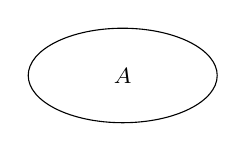
\begin{tikzpicture}[scale=.6,font=\footnotesize,line join=round,line cap=round,>=stealth]
					\draw (3,0)  arc (0:360:2 cm and 1 cm);
					 \draw (1,0) node{$A$};
				\end{tikzpicture}
			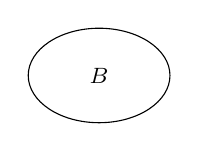
\begin{tikzpicture}[scale=.6,font=\footnotesize,line join=round,line cap=round,>=stealth]
					\draw (5,0) arc  (0:360:1.5 cm and 1 cm);
					\draw (3.5,0)  node{$B$};
				\end{tikzpicture}
		\end{center}
		\begin{center}
			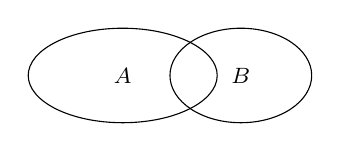
\begin{tikzpicture}[scale=.6,font=\footnotesize,line join=round,line cap=round,>=stealth]
					\draw (3,0) arc (0:360:2 cm and 1  cm);
					 \draw (5,0) arc (0:360:1.5 cm and 1 cm);
					 \draw (1,0) node{$A$};
					 \draw (3.5,0) node{$B$};
				\end{tikzpicture}
		\end{center}
		 Kiểm tra các đáp án bằng cách vẽ biểu đồ Ven cho hai trường hợp $A\cap B=\varnothing$ và $A\cap B\neq \varnothing$.
	} 
\end{ex}

% nguồn: MaHoaNH_TracNghiem_Lop10
\begin{ex}%[0D1V3-1]%[ma:32f8d3fa]
	Cho hai tập hợp $A=\{0;2\}$ và  $B=\{0;1;2;3;4\}$. Số tập hợp $X$ thỏa mãn $A\cup X=B$ là
	 \choice
		{$2$} 
		{\True $3$} 
		 {$4$}
		{$5$} 
	\loigiai{ 
		\begin{center}
			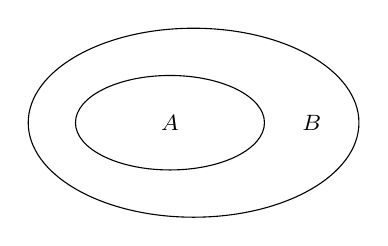
\begin{tikzpicture}[scale=.6,font=\footnotesize,line join=round,line cap=round,>=stealth]
					\draw (0,0) ellipse (2cm and 1cm) 
						 (0,0) node{$A$};
					\draw (0.5,0)  ellipse (3.5cm and 2cm)
						(3,0) node{$B$}; 
				\end{tikzpicture}
		\end{center}
		$A\cup X=B$ nên bắt buộc $X$  phải chứa các phần tử $\{1;3;4\}$ và $X\subset B$.\\
		Vậy  $X$ có $3$ tập hợp đó là $\{1;3;4\},\{1;2;3;4\},\{0;1;2;3;4\}$.
	} 
\end{ex}

% nguồn: MaHoaNH_TracNghiem_Lop10
\begin{ex}%[0D1K3-1]%[ma:b39a2054]
	Với giả thiết nào dưới đây thì có thể  kết luận $A\cap B=A\cup B$?
	\choice{$A \setminus B= \varnothing  $}
		{$B  \subset A $}
		 {$A \subset B $}
		{\True $A=B$} 
	\loigiai{Khi  $A=B$ thì $A\cap B=A\cap A=A$ và $A\cup B=A\cup A=A$. Do đó $A\cap B=A\cup B$.}
\end{ex}

% nguồn: MaHoaNH_TracNghiem_Lop10
\begin{ex}%[0D1B3-1]%[ma:e554ef66]
	Cho hai tập hợp $A=\{1; 2; 3; 4; 5\}$ và  $B=\{0; 2; 4\}$. Xác định $A\cup B$.
	 \choice
		{\True $\{0; 1; 2;  3; 4; 5\}$}
		 {$\{0\}$}
		{$\varnothing$} 
		{$\{2;4\}$} 
	\loigiai{Ta  có $A\cup B=\{0; 1; 2; 3; 4; 5\}$.}
\end{ex}

% nguồn: MaHoaNH_TracNghiem_Lop10
\begin{ex}%[0D1K3-1]%[ma:e638b7df]
	Cho tập hợp $B = \left\{x \in \mathbb{N}^* \big| x \leq 4\right\}$ và tập  hợp $A$ gồm những số tự nhiên lẻ không lớn hơn $8$. Tìm tập hợp $A \cap B$.
	 \choice
		{\True $\left\{1,  3\right\}$}
		{$\left\{1, 2, 3, 4\right\}$} 
		{$\left\{0, 1,  3, 5\right\}$}
		{$\left\{0, 1, 2, 3, 4, 5,  7\right\}$}
	\loigiai{$A = \left\{1, 3, 5, 7\right\}; B = \left\{1, 2, 3, 4\right\}$. Nên $A \cap B = \left\{1, 3\right\}$.} 
\end{ex}

% nguồn: MaHoaNH_TracNghiem_Lop10
\begin{ex}%[0D1K3-1]%[ma:ab7dd9e5]
	Cho tập  hợp $A =\left\{x \in \mathbb{R} \big| (x^2 -1)(x^2 - 4) = 0\right\}$ và tập hợp $B = \left\{x \in \mathbb{Z} \big| |x| \leq 2 \right\}$. Khi đó, tập $A \cup B$ là
	\choice 
		{\True $\left\{-2, -1, 0,  1, 2\right\}$}
		{$\left\{-4, -2, -1, 0, 1,  2, 4\right\}$}
		{$\left\{-2,  -1, 1, 2\right\}$}
		{$\left\{-2, 0,  2\right\}$}
	\loigiai{$A = \left\{-2, -1, 1, 2\right\}, B = \left\{-2, -1, 0, 1, 2\right\}$. Nên $A \cup B = \left\{-2, -1,  0, 1, 2\right\}$}
\end{ex}

% nguồn: MaHoaNH_TracNghiem_Lop10
\begin{ex}%[0D1B3-1]%[ma:a8d28870]
	Cho hai  tập hợp $A=\{1;5\}$ và $B=\{1;3;5\}$. Chọn kết quả đúng trong các kết quả sau
	 \choice
		 { $A \cap B=\{1\}$}
		 {$A \cap B=\{1;3\}$}
		 {\True $A \cap B=\{1;5\}$}
		{$A \cap  B=\{1;3;5\}$}
	\loigiai{Ta có $A \cap B=\{1;5\}$. 
	 }
\end{ex}

% nguồn: MaHoaNH_TracNghiem_Lop10
\begin{ex}%[0D1B3-1]%[ma:661b8c21]
	Cho $A=\{1;5\}$, $B=\{1;3;5\}$. Chọn kết quả đúng trong các  kết quả sau.
	 \choice
		{$A  \cup B=\{3;5\}$}
		{$A  \cup B=\{1;3\}$}
		{$A  \cap B=\{1\}$}
		{\True $A \cap  B=\{1;5\}$}
	 \loigiai{
	 Ta có $A \cap B=\{1;5\}$.}
\end{ex}

% nguồn: MaHoaNH_TracNghiem_Lop10
\begin{ex}%[0D1B3-1]%[ma:4ea55379]
	 Cho $A=(-\infty;5]$, $B=(0;+\infty)$. Tìm $A\cap B$.
	\choice 
		{$A\cap B=[0;5)$} 
		{$A\cap B=(0;5)$} 
		{\True $A\cap B=(0;5]$} 
		 {$A\cap B=(-\infty;+\infty)$}
	 \loigiai{
	 $A\cap B$ $=(0;5]$.}
\end{ex}

% nguồn: MaHoaNH_TracNghiem_Lop10
\begin{ex}%[0D1K3-1]%[ma:fb80aa37]
	Cho $A=(-\infty;m+1]$; $B=(-1;+\infty)$. Điều  kiện để $A\cup B=\mathbb{R}$ là
	\choice 
		 {$m>-1$}
		 {\True $m\geqslant -2$}
		{$m\geqslant 0$} 
		 {$m>-2$}
	 \loigiai{
	Ta  có: $\left(A\cup B\right)=\mathbb{R}$ $ \Leftrightarrow -1\leqslant m+1 \Leftrightarrow m\geqslant -2$.}
\end{ex}

% nguồn: MaHoaNH_TracNghiem_Lop10
\begin{ex}%[0D1B3-1]%[ma:c3998f6d]
	 Cho $A=(-\infty;2]$, $B=[2;+\infty)$, $C=(0;3)$. Chọn phát biểu \textbf{sai}.
	 \choice
		{$A\cap C=(0;2]$} 
		 {$B\cup C=(0;+\infty)$}
		{\True $A\cup  B=\mathbb{R}\setminus \{2\}$}
		 {$B\cap C=[2;3)$}
	\loigiai{ 
	Ta có: $A\cup  B=\mathbb{R}$.}
\end{ex}

% nguồn: MaHoaNH_TracNghiem_Lop10
\begin{ex}%[0D1B3-1]%[ma:6ba0160a]
	Cho $M=\lbrace 0;1;2;3;4 \rbrace$ và $N= \lbrace 0;2;4;6;8 \rbrace$. Khi đó tập hợp $M \cap  N$ là
	\choice{$\lbrace 6;8 \rbrace  $}
		{$\lbrace 1;3  \rbrace$}
		{\True $ \lbrace 0;2;4 \rbrace$} 
		{$\lbrace  0;1;2;3;4;6;8 \rbrace $}
	\loigiai{$M \cap  N=\{x|x\in M \text{ và } x\in N\}$.\\
		Từ giả thiết,  ta có $M \cap N=\{0;2;4\}$.
	 }
\end{ex}

% nguồn: MaHoaNH_TracNghiem_Lop10
\begin{ex}%[0D1B3-1]%[ma:9317f0b1]
	Cho tập hợp $X=(-\infty;2] \cap (-6;+\infty)$. Khẳng định  nào sau đây là đúng?
	 \choice
		{\True $X=(-6;2]$} 
		 {$X=(-\infty;+\infty)$}
		 {$(-6;+\infty)$}
		{$X=(-\infty;2]$} 
	 \loigiai{
	Ta  có: $X=(-\infty;2] \cap (-6;+\infty)=(-6;2]$.}
\end{ex}

% nguồn: MaHoaNH_TracNghiem_Lop10
\begin{ex}%[0D1B3-1]%[ma:e67d8752]
	Cho $A=\left(1;9\right)$, $B=[3;+\infty)$, câu nào sau đây đúng? 
	 \choice
		 {$A\cap B=[1;+\infty)$}
		{$A\cap  B=(9;+\infty)$}
		 {$A\cap B=(1;3)$}
		{\True  $A\cap B=[3;9)$}
	 \loigiai{
	 $$A\cap B=\left(1;9\right)\cap \left[3;+\infty \right)=\left[3;9\right).$$}
\end{ex}

% nguồn: MaHoaNH_TracNghiem_Lop10
\begin{ex}%[0D1B3-1]%[ma:46bd2d6d]
	Cho tập  hợp $A=\{1;2;3;5;7\}$, $B=\{2;4;5;6;8\}$. Tập hợp $A \cap B$ là
	 \choice
		{$\{5\}$} 
		 {$\{2\}$}
		 {$\{1;2;3;4;5;6;7;8\}$}
		 {\True $\{2;5\}$}
	\loigiai{Ta  có $A \cap B=\{2;5\}$.
	} 
\end{ex}

% nguồn: MaHoaNH_TracNghiem_Lop10
\begin{ex}%[0D1Y3-1]%[ma:5b8094e6]
	Cho hai tập  hợp $A=(-3;3)$, $B=[-1;5]$. Tìm $A \cup B$?
	\choice 
		 {$[-1;3)$}
		{$(-3;-1]$} 
		 {$(3;5]$}
		{\True $(-3;5]$} 
	\loigiai{ 
	Ta có $A  \cup B=(-3;5]$.}
\end{ex}

% nguồn: MaHoaNH_TracNghiem_Lop10
\begin{ex}%[0D1B3-1]%[ma:05d4a6b6]
	 Cho $X=\{7;2;8;4;9;12\}$; $Y=\{ 1;3;7;4\}$. Tập hợp nào sau đây bằng $X\cap Y$?
	\choice 
		{  $\{1;2;3;4;8;9;7;12\}$}
		 {$\{2;8;9;12\}$}
		{\True  $\{4;7\}$}
		 {$\{1;3\}$}
	\loigiai{Ta có $X\cap Y=\{4;7\}$. 
	} 
\end{ex}

% nguồn: MaHoaNH_TracNghiem_Lop10
\begin{ex}%[0D1B3-1]%[ma:c630b4c5]
	Cho hai đa thức $f(x)$ và $g(x)$. Xét các tập hợp $A=\{x\in\mathbb{R}\;\big|\;f(x)=0\}$, $B=\{x\in\mathbb{R}\;\big|\;g(x)=0\}$ và $C=\{x\in\mathbb{R}|f^2(x)+g^2(x)=0\}$. Trong các mệnh đề sau, mệnh đề nào là mệnh  đề đúng?
	\choice 
		{$C=A\cup B$} 
		{\True $C=A\cap  B$}
		{$C=A\setminus  B$}
		{$C=B\setminus  A$}
	\loigiai{Ta có $f^2(x)+g^2(x)=0  \Leftrightarrow \heva{&f(x)=0\\&g(x)=0.}$\\
	Do đó  $C=A\cap B$.}
\end{ex}

% nguồn: MaHoaNH_TracNghiem_Lop10
\begin{ex}%[0D1B3-1]%[ma:61c6ce3c]
	Cho $A=\left\{x\in \mathbb{N}\;|\;x\leqslant 3\right\}$, $B=\{0;1;2;3\}$. Tập $A\cap B$  bằng
	 \choice
		{$\{1;2;3\}$} 
		{$\{-3;-2;-1;0;1;2;3\}$} 
		{$\{0;1;2\}$} 
		{\True $\{0;1;2;3\}$} 
	\loigiai{ 
	$A=\left\{x\in \mathbb{N}\;|\;x\leqslant 3\right\}=\{0; 1; 2; 3\}$ $ \Rightarrow A\cap B=\{0;  1; 2; 3\}$.}
\end{ex}

% nguồn: MaHoaNH_TracNghiem_Lop10
\begin{ex}%[0D1Y3-1]%[ma:c7eb16e6]
	Cho hai tập hợp $X=\{-1;1;3;5;8\}$; $Y=\{3;5;7;9\}$. Tập hợp $X\cup Y$ bằng tập  hợp nào sau đây?
	 \choice
		{$\{3;5\}$} 
		{$\{1;7;9\}$} 
		{$\{1;3;5\}$} 
		 {\True $\{-1;1;3;5;7;8;9\}$}
	\loigiai{ 
		 Ta có $X\cup Y=\{-1;1;3;5;7;8;9\}$.
	 }
\end{ex}

% nguồn: MaHoaNH_TracNghiem_Lop10
\begin{ex}%[0D1K3-1]%[ma:7c04d734]
	Cho các tập hợp $A=\left\{a,b\right\}$, $B=\left\{1,2,3\right\}$, $C=\left\{b,c\right\}$ và $D=\left\{2,3,4\right\}$, trong đó $a, b, c\in\mathbb{R}$ và $a$, $b$, $c\notin B,D$ là các phần tử khác nhau từng đôi một. Tìm tập hợp  $E=\left(A\cap B\right)\cup\left(C\cap D\right)$.
	\choice 
		 {$E=\left\{a,c\right\}$}
		 {$E=\left\{b,2\right\}$}
		 {\True $E=\varnothing$}
		{$E=\left\{b,2,3\right\}$} 
	\loigiai{ 
		Ta có $\heva{&  A\cap B=\varnothing\\ & C\cap D=\varnothing}\Rightarrow E=\left(A\cap B\right)\cup\left(C\cap D\right)=\varnothing$.
	 }
\end{ex}

% nguồn: MaHoaNH_TracNghiem_Lop10
\begin{ex}%[0D1K3-1]%[ma:848e9758]
	Cho hai tập hợp $A=\left\{x\in \mathbb{R}\big|\left(x^2-1 \right)\left(x^2-3x+4  \right)=0 \right\}$ và $B=\left\{x\in \mathbb{Z}\big|\left| x \right|\leq 2 \right\}$. Tìm tập hợp $A\cup B$.
	\choice 
		 {\True $\left\{-2,-1,0,1,2 \right\}$}
		{$\left\{-2,-1,0,1,2, -4  \right\}$}
		{$\left\{-1, 1  \right\}$}
		{$\left\{-2, 0,  2\right\}$}
	 \loigiai{
		Ta có $A=\left\{-1, 1\right\}, B=\left\{-2, -1, 0, 1,  2\right\}$. Suy ra $A\cup B =\left\{-2, -1, 0, 1, 2\right\}$.
	} 
\end{ex}

% nguồn: MaHoaNH_TracNghiem_Lop10
\begin{ex}%[0D1Y3-1]%[ma:d4414e61]
	Cho dãy số liệu $1; 3; 4; 6; 8; 9; 11$.  Số trung bình cộng của dãy số liệu trên?
	 \choice
		 {$ 11 $}
		{\True  $ 6 $ }
		{$ 9 $} 
		{$  5 $}
	\loigiai{ 
		Số  trung bình cộng của dãy số liệu trên là $ \overline{x}=\dfrac{1+3+4+6+8+9+11}{7}= 6$.
	 }
\end{ex}

% nguồn: MaHoaNH_TracNghiem_Lop10
\begin{ex}%[0D1K3-1]%[ma:6a6818db]
	Cho các tập hợp $A=\left\{a,b\right\}$, $B=\left\{1,2,3\right\}$, $C=\left\{b,c\right\}$ và $D=\left\{2,3,4\right\}$, trong đó $a, b, c\in\mathbb{R}$ và $a$, $b$, $c\notin B,D$ là các phần  tử khác nhau từng đôi một. Tìm tập hợp $E=\left(A\cup B\right)\cap\left(C\cup D\right)$.
	\choice 
		{$E=\left\{a,2,3\right\}$} 
		 {\True $E=\left\{b,2,3\right\}$}
		 {$E=\left\{2,3,4\right\}$}
		 {$E=\left\{a,b,c\right\}$}
	 \loigiai{
		Ta có $\heva{& A\cup B=\left\{a,b,1,2,3\right\}\\ & C\cup D=\left\{b,c,2,3,4\right\}}\Rightarrow  E=\left(A\cup B\right)\cap\left(C\cup D\right)=\left\{b,2,3\right\}$.
	 }
\end{ex}

% nguồn: MaHoaNH_TracNghiem_Lop10
\begin{ex}%[0D1B3-1]%[ma:047fed31]
	Chọn kết quả  sai trong các kết quả dưới đây.
	 \choice
		{\True $[-3; 1)  \cup(-5; 3)=[-3; 3)$}
		{$[-3;  1) \cup(-2; 3)=[-3; 3)$}
		{$[-3; 1)  \cup(-4; 3)=(-4; 3)$}
		{$[-3; 1)  \cup(-3; 3)=[-3; 3)$}
	 \loigiai{
		$[-3; 1)  \cup(-5; 3)=[-5; 3)$
	} 
\end{ex}

% nguồn: MaHoaNH_TracNghiem_Lop10
\begin{ex}%[0D1B3-1]%[ma:c9b0c9f7]
	Cho hai tập hợp $A=\left\{a; b; 1;  2\right\}$ và $B=\left\{a; b; c; 1; 3\right\}.$ Tìm tập hợp $A\cap B.$
	\choice 
		{\True  $A\cap B=\left\{a,b,1\right\}$}
		{$A\cap  B=\left\{a,b,2\right\}$}
		{$A\cap B=\left\{a,b,3\right\}$} 
		{$A\cap B=\left\{2,3,c\right\}$} 
	\loigiai{ 
		$A\cap B=\{x\,|\,x\in A \text{ và } x\in B\}$. Vậy theo  giả thiết $A\cap B=\left\{a,b,1\right\}$.
	} 
\end{ex}

% nguồn: MaHoaNH_TracNghiem_Lop10
\begin{ex}%[0D1B3-1]%[ma:fec93c7e]
	Cho $M=(-\infty; 5]$ và $N=[-2; 6)$. Hãy  tìm $M \cap N$.
	 \choice
		 {\True $M \cap N=[-2; 5]$}
		{$M  \cap N=(-\infty, 6)$}
		{$M \cap N=(-2;-5)$} 
		{$M \cap  N=[-2; 6)$}
	 \loigiai{
		$M  \cap N=[-2; 5]$
	 }
\end{ex}

% nguồn: MaHoaNH_TracNghiem_Lop10
\begin{ex}%[0D1B3-1]%[ma:d3fc5d61]
	Cho hai tập hợp $M,N$ thoả mãn $M \subset N$. Mệnh đề nào sau đây là  đúng?
	 \choice
		 {$M \setminus N=M$}
		{\True $M \cap  N=N$}
		{$M \cap N=M$} 
		{$M  \setminus N=N$}
	\loigiai{ 
		Vì $M$ chứa trong $N$ nên $M  \cap N =N$.
	 }
\end{ex}

% nguồn: MaHoaNH_TracNghiem_Lop10
\begin{ex}%[0D1B3-1]%[ma:a97e4b36]
	Cho hai tập hợp $A=\left\{1;2;3;4\right\}$, $B=\left\{ 2;4;6;8 \right\}$. Tập hợp nào sau đây  bằng tập hợp $A\cap B$?
	 \choice
		{\True$\left\{ 2;4  \right\}$}
		 {$\left\{1;2;3;4;6;8 \right\}$}
		{$\left\{6;8  \right\}$}
		 {$\left\{1;3 \right\}$}
	\loigiai{ 
		Ta có $A\cap B=\left\{ 2;4 \right\}.$ 
	 }
\end{ex}

% nguồn: MaHoaNH_TracNghiem_Lop10
\begin{ex}%[0D1K3-1]%[ma:5c6652a8]
	Cho $A=\left[- 3; 5\right]$ và $B=\left(-\infty;-2\right) \cup\left(1;+\infty\right)$. Khi đó $A \cap  B$ là
	\choice 
		 {$\left(-\infty,-2\right] \cup\left(1;+\infty\right)$}
		 {$\left(-\infty;-2\right) \cup\left[1;+\infty\right)$}
		 {\True $\left[-3;-2\right) \cup\left(1; 5\right]$}
		{$\left[-3;-2\right)  \cup\left(1; 5\right)$}
	\loigiai{ 
		$A \cap B=  \left[-3;-2\right) \cup\left(1; 5\right] $
	 }
\end{ex}

% nguồn: MaHoaNH_TracNghiem_Lop10
\begin{ex}%[0D1B3-1]%[ma:65803861]
	Biết điểm $M\left(1;-2\right)$ biểu diễn số phức $z$ trong mặt phẳng toạ độ  phức. Tính mô-đun của số phức $w=\overline{iz}-z^2$.
	 \choice
		{\True  $\sqrt{26}$}
		 {$\sqrt{25}$}
		{$\sqrt{24}$} 
		{$\sqrt{23}$} 
	 \loigiai{
		Vì điểm $M\left(1;-2\right)$ biểu diễn số phức  $z$ nên $z=1-2i \Rightarrow \overline{z}=1+2i$.\\
		 Do đó $w=\overline{iz}-z^2=i\left(1+2i\right)-\left(1-2i\right)^2=-2+i-\left(-3-4i\right)=1+5i \Rightarrow \left|w\right|=\sqrt{26}$.
	 }
\end{ex}

% nguồn: MaHoaNH_TracNghiem_Lop10
\begin{ex}%[0D1K3-1]%[ma:c7f5a61f]
	Tập hợp nào dưới đây là  giao của hai tập hợp $A=\left\{x\in \mathbb{R}\colon -1\leqslant x<3\right\}$,\\$B=\left\{x\in \mathbb{R}\colon |x|<2\right\}$ ?
	 \choice
		{$(-1;2)$} 
		 {$[0;2)$}
		{$(-2;3)$} 
		 {\True $[-1;2)$}
	 \loigiai{
		Ta viết lại hai tập hợp như sau: $A=\left\{x\in \mathbb{R}\colon -1\leqslant  x<3\right\}=[-1;3)$.
		\[B=\left\{x\in \mathbb{R}\colon |x|<2\right\}=(-2;2).\] 
	Suy ra $A\cap  B=[-1;2)$.}
\end{ex}

% nguồn: MaHoaNH_TracNghiem_Lop10
\begin{ex}%[0D1Y3-1]%[ma:7d584b0a]
	Cho hai tập khác rỗng $A=(m-1;4]$, $B=(-2;2m+2)$ với $m \in  \mathbb{R}$. Xác định $m$ để $A \cap B \ne \varnothing$.
	 \choice
		{\True $-2<m<5$} 
		 {$m<5$}
		 {$m>-3$}
		 {$-3<m<5$}
	\loigiai{ 
		$A$ và $B$ là hai tập hợp khác rỗng nên  $$\heva{&m-1<4 \\& 2m+2>-2}\Leftrightarrow \heva{&m<5 \\& m>-2}\Leftrightarrow -2<m<5 \quad (1).$$
		Để $A \cap B \ne \varnothing$  thì $$m-1<2m+2 \Leftrightarrow m>-3 \quad (2).$$
	 Từ (1) và (2) suy ra $-2<m<5$.}
\end{ex}

% nguồn: MaHoaNH_TracNghiem_Lop10
\begin{ex}%[0D1B3-1]%[ma:8a93a3fe]
	Cho hai tập hợp $ A=\left\lbrace x\in \mathbb{R}\,\mid\,(2x-x^2)(x-1)=0 \right\rbrace$, $ B=\left\lbrace n \in \mathbb{N}\,\mid\,0<n^2<10 \right\rbrace$. Chọn  mệnh đề đúng?
	 \choice
		{\True  $A \cap B =\left\lbrace 1;2 \right\rbrace $}
		{$A \cap B  =\left\lbrace 2 \right\rbrace $}
		{ $A \cap B =\left\lbrace 0;1;2;3  \right\rbrace $}
		{$A \cap  B =\left\lbrace 0;3 \right\rbrace $}
	\loigiai{ 
		 Ta có
		\begin{itemize}
			\item $ (2x-x^2)(x-1)=0\Leftrightarrow \hoac{& x=0\\  &x=1\\&x=2 }\Rightarrow A=\left\lbrace 0;1;2 \right\rbrace $.
			\item $ B=  \left\lbrace 1;2;3 \right\rbrace$.
		\end{itemize}
	Suy ra  $ A\cap B= \left\lbrace 1;2 \right\rbrace$.}
\end{ex}

% nguồn: MaHoaNH_TracNghiem_Lop10
\begin{ex}%[0D1B3-1]%[ma:716746ac]
	Cho  các tập hợp sau:\\
	$A=\{x\in\mathbb{R}\mid (x-2x^2)(x^2-3x+2)=0\}$;\\ $B=\{n\in\mathbb{N}\mid 3<n(n+1)<31\}$.\\ 
	Khi đó 
	\choice 
		{$A\cap  B=\{2;4\}$}
		{$A\cap B=\{4;5\}$} 
		{\True  $A\cap B=\{2\}$}
		{$A\cap  B=\{3\}$}
	 \loigiai{
		Ta  có:\\
		$x\in  A \Leftrightarrow (x-2x^2)(x^2-3x+2)=0\Leftrightarrow \hoac{&x-2x^2=0\\&x^2-3x+2=0}\Leftrightarrow \hoac{&x=0\\&x=2\\&x=1.}$\\
		 Do đó, ta có: $A=\{0;1;2\}$.\\
		Thử trực tiếp với các  giá trị $n\in\mathbb{N}$, ta có: $B=\{2;3;4;5\}$.\\
	Vậy $A\cap  B=\{2\}$.}
\end{ex}

% nguồn: MaHoaNH_TracNghiem_Lop10
\begin{ex}%[0D1B3-1]%[ma:d09611e9]
	Cho các tập hợp $A=\left\{ x\in \mathbb{N} \ | \ (4-x^2)(x^2-5x+4)=0 \right\}; B = \left\{ x\in \mathbb{Z} \ | \  x \text{ là ước của } 4 \right\}$. Tập hợp $A \cap B$ là
	\choice 
		{$\{-2,1,2,4\}$} 
		 {\True $\{1,2,4\}$}
		{$\{2,4\}$} 
		{$\{-4,-2,-1,1,2,4\}$} 
	\loigiai{ 
		Ta có $(4-x^2)(x^2-5x+4)=0 \Leftrightarrow  \hoac{&4-x^2=0\\&x^2-5x+4=0} \Leftrightarrow \hoac{&x=2\\&x=-2\\&x=1\\&x=4.}$\\
		Vì $x\in \mathbb{N}$ nên $x  \in \{1,2,4\}$.\\
		Do đó $A=\{1,2,4\} \quad (1)$.\\ 
		Ta có các ước của  $4$ là $\pm 1, \pm 2, \pm 4$.\\
		 Do đó $B=\{-4,-2,-1,1,2,4\} \quad (2)$.\\
		Từ $(1), (2)$ ta có  $A \cap B = \{1,2,4\}$.
	 }
\end{ex}

% nguồn: MaHoaNH_TracNghiem_Lop10
\begin{ex}%[0D1B3-1]%[ma:5644c6ae]
	Chọn  khẳng định \bf{sai} trong các khẳng định sau
	 \choice
		 {$\mathbb{Q} \cup \mathbb{R}=\mathbb{R}$}
		 {$\mathbb{N} \cap \mathbb{Z}=\mathbb{N}$}
		 {$\mathbb{Q} \cap \mathbb{N}^{\star}=\mathbb{N}^{\star}$}
		{\True $\mathbb{Q}  \cup \mathbb{N}^{\star}=\mathbb{N}^{\star}$}
	\loigiai{Ta có $\mathbb{N}^{\star} \subset \mathbb{N} \subset \mathbb{Z} \subset \mathbb{Z} \subset  \mathbb{Q}$. Do đó
		\begin{itemize}
			 \item $\mathbb{Q} \cup \mathbb{R}=\mathbb{R}$ đúng;
			 \item $\mathbb{N} \cap \mathbb{Z}=\mathbb{N}$ đúng;
			\item $\mathbb{Q} \cap \mathbb{N}^{\star}=\mathbb{N}^{\star}$  đúng;
			\item $\mathbb{Q} \cup \mathbb{N}^{\star}=\mathbb{N}^{\star}$  sai.
		\end{itemize}
	 }
\end{ex}

% nguồn: MaHoaNH_TracNghiem_Lop10
\begin{ex}%[0D1K3-1]%[ma:625cc90d]
	Để phục vụ cho hội nghị  quốc tế, ban tổ chức cần huy động các phiên dịch viên tiếng Anh và
	tiếng Pháp. Biết rằng trong những  người này có $25$ người phiên dịch được tiếng Anh, $12$ người phiên dịch
	được  tiếng Pháp, trong đó có $8$ người phiên dịch được cả hai thứ tiếng. Hỏi ban tổ chức đã huy động tất
	cả bao  nhiêu phiên dịch viên?
	 \choice
		{$45$} 
		{$37$} 
		{$33$} 
		{\True  $29$}
	 \loigiai{
		\begin{itemize}
			\item Số người chỉ phiên dịch được  tiếng Anh là $S_1=25-8=17$ người.
			\item Số người chỉ phiên dịch được tiếng  Pháp là $S_2=12-8=4$ người.
			\item Số người phiên dịch được cả tiếng  Anh và tiếng Pháp là $S_3=8$ người.
		\end{itemize}
	Vậy ban tổ chức đã  huy động tất cả $S=S_1+S_2+S_3=17+4+8=29$ người.}
\end{ex}

% nguồn: MaHoaNH_TracNghiem_Lop10
\begin{ex}%[0D1Y3-1]%[ma:c73d10b8]
	Điểm kiểm tra môn  Văn của một nhóm gồm $7$ học sinh như sau:
	$$ 
	\begin{array}{llllllll}
		5 & 6 & 8 & 6 & 7  & 8 & 5
	\end{array}
	$$ 
	Điểm trung bình môn Văn của $7$ học sinh đó (kết quả làm  tròn đến hàng phần mười) là
	 \choice
		{$6{,}2$} 
		{\True  $6{,}4$}
		 {$6{,}6$}
		 {$6{,}7$}
	\loigiai{ 
		 Điểm trung bình môn Văn của $7$ học sinh đó là
		$$\bar  x=\dfrac{5+6+8+6+7+8+5}{7}=6{,}4.$$
	 }
\end{ex}

% nguồn: MaHoaNH_TracNghiem_Lop10
\begin{ex}%[0D1B3-1]%[ma:4a49de2c]
	 Cho tập hợp $ A $. Chọn khẳng định đúng.
	 \choice
		{$ A\cap \varnothing  = A $}
		{\True $  A \cup \varnothing = A $}
		 {$\varnothing\not\subset A$}
		{$\left\lbrace \varnothing\right\rbrace\subset A$} 
	\loigiai{ 
	 Ta có
	\begin{itemize}
		\begin{multicols}{2}
			\item  $ A\cap \varnothing = \varnothing $.
			\item $ A\cup  \varnothing=A $.
			\item $\varnothing\subset A, \,  \forall A$.
			\item Tập $ \left\lbrace \varnothing \right\rbrace  $ không là tập con của tập $ A $.
		\end{multicols}
	\end{itemize}
	} 
\end{ex}

% nguồn: MaHoaNH_TracNghiem_Lop10
\begin{ex}%[0D1K3-1]%[ma:fe18fdea]
	Cho $2$ tập hợp $A=\left\{x\in \mathbb{R}\;|\;(2x-x^2)(2x^2-3x-2)=0\right\}$,\\ $B=\left\{n\in \mathbb{N}\;|\;3<n^2<30\right\}$, chọn mệnh đề đúng? 
	\choice 
		{\True $A\cap B=\{2\}$} 
		 {$A\cap B=\{5;4\}$}
		 {$A\cap B=\{2;4\}$}
		 {$A\cap B=\{3\}$}
	 \loigiai{
		Xét tập hợp $A=\left\{x\in \mathbb{R}\;|\;(2x-x^2)(2x^2-3x-2)=0\right\}$ ta có \[(2x-x^2)(2x^2-3x-2)=0 \Leftrightarrow \left[\begin{aligned}
		 &2x-x^2=0\\
		&2x^2-3x-2=0\\ 
	\end{aligned}\right. \Leftrightarrow \left[\begin{aligned}
	 &x=0\\
	&x=-\dfrac{1}{2}\\ 
	&x=2\\ 
	\end{aligned}\right. \Rightarrow A=\left\{0;2;-\dfrac{1}{2}\right\}.\]\\
	Xét tập hợp $B=\left\{n\in \mathbb{N}|3<n^2<30\right\}$  $=\{2;3;4;5\}$.\\
Vậy $A\cap  B=\{2\}$.}
\end{ex}

% nguồn: MaHoaNH_TracNghiem_Lop10
\begin{ex}%[0D1Y3-1]%[ma:5c4f8a9d]
	Lớp $ 10C $ của một trường trung học phổ thông có điểm thi môn Toán được cho dưới bảng sau 
	\begin{center}
		\begin{tabular}{|l|c|c|c|c|c|c|}
			\hline Điểm thi & 5 &  6 & 7 & 8 & 9 & 10 \\
			 \hline Tần số & 5 & 7 & 12 & 14 & 3 & 4 \\
			\hline 
		\end{tabular}
	\end{center}
	Tính điểm trung  bình cộng môn Toán của lớp $10C$ (làm tròn đến hàng phần mười)?
	 \choice
		{$  8 $}
		{$ 7,5 $  }
		 {$ 7,6 $}
		{\True  $ 7,3 $}
	\loigiai{ 
		Điểm trung bình của lớp $  10 C $ là
		$ \overline{x}=\dfrac{5\cdot 5+7\cdot 6+12\cdot 7+14\cdot 8+3\cdot 9+4\cdot10}{45} \approx 7,3$. 
	} 
\end{ex}

% nguồn: MaHoaNH_TracNghiem_Lop10
\begin{ex}%[0D1K3-1]%[ma:bcb6251b]
	Cho  hai tập hợp $A=[1-2m;m+3]$, $B=\left\{x\in \mathbb{R}\mid x\geqslant 8-5m\right\}$ với $m$ là một tham số thực. Tìm tất cả các giá trị $m$ để $A\cap B=\varnothing$.
	\choice 
		{$m\geqslant  \dfrac{5}{6}$}
		 {$m<-\dfrac{2}{3}$}
		{$m\leqslant  \dfrac{5}{6}$}
		{\True $-\dfrac{2}{3}\leqslant m<\dfrac{5}{6}$} 
	 \loigiai{
		Ta có $A=[1-2m;m+3]$,  $B=[8-5m;+\infty)$.\\
		$A\cap B=\varnothing $ $ \Leftrightarrow $ $\left\{\begin{aligned}
		&m+3<8-5m\\ 
		 &1-2m\leqslant m+3\\
	\end{aligned}\right. $ $ \Leftrightarrow $ $\left\{\begin{aligned}
	&6m<5\\ 
	&3m\geqslant -2\\ 
	\end{aligned}\right. $ $ \Leftrightarrow $ $\left\{\begin{aligned}
	&m<\dfrac{5}{6}\\ 
	 &m\geqslant -\dfrac{2}{3}\\
	\end{aligned}\right. $ $ \Leftrightarrow $ $-\dfrac{2}{3}\leqslant m<\dfrac{5}{6}$.}
\end{ex}

% nguồn: MaHoaNH_TracNghiem_Lop10
\begin{ex}%[0D1B3-1]%[ma:cabe843a]
	Cho hai tập $A=\left\{ x\in \mathbb{R}  \,\mid\,(x^2-4x+3)(x^2-4)=0 \right\}$ và $B=\left\{ x\in \mathbb{N} \,\mid\, x<4 \right\}$. Tìm $A\cap B$.
	\choice 
		 { $A\cap B=\left\{ -2;1;2 \right\}$}
		{  $A\cap B=\left\{ 0;1;2;3 \right\}$}
		{  \True $A\cap B=\left\{ 1;2;3 \right\}$}
		{ $A\cap B=\left\{ -1;2  \right\}$}
	\loigiai{ 
		Ta có $(x^2-4x+3)(x^2-4)=0  \Leftrightarrow \hoac{
		 & x=1\\
		 & x=3\\
		& x=2\\ 
		&  x=-2
		} \Rightarrow A=\left\{  -2;1;2;3 \right\}$.\\
		 Ta có $\heva{
		&  x\in \mathbb{N}\\
		 & x<4\\
		} \Rightarrow B=\left\{0;1;2;3  \right\}$.\\
		Suy ra $A\cap B=\left\{ 1;2;3 \right\}$. 
	 }
\end{ex}

% nguồn: MaHoaNH_TracNghiem_Lop10
\begin{ex}%[0D1B3-1]%[ma:4cf07506]
	Cho hai tập  hợp $A=[-2;3]$ và $B=(1;+\infty)$. Tìm $A\cap B$.
	 \choice
		{$A\cap  B=[-2;+\infty)$}
		 {\True $A\cap B=(1;3]$}
		{$A\cap B=[1;3]$} 
		 {$A\cap B=(1;3)$}
	\loigiai{ 
		Biểu diễn hai tập hợp $A$ và $B$ ta  được:
		\begin{center}
			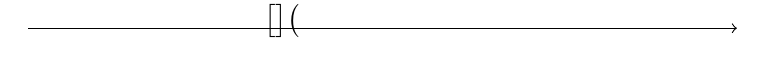
\begin{tikzpicture}
					\draw[->](-3,0)->(6,0); 
					 \IntervalLR{-3}{-2}
					\IntervalGR{}{}{\big[}{-2} 
					 \IntervalLR{3}{5.9}
					\IntervalGR{\big]}{3}{}{} 
					 \IntervalLR{-3}{1}
					 \IntervalGL{}{}{\big (}{1}
				\end{tikzpicture}
		\end{center}
		Vậy $A\cap B=(1;3]$. 
	 }
\end{ex}

% nguồn: MaHoaNH_TracNghiem_Lop10
\begin{ex}%[0D1Y3-1]%[ma:8f5592ea]
	Cho hai tập hợp $E=(-\infty;6]$ và $F=[-2;7]$.  Khi đó $E\cap F$ là
	 \choice
		{\True $E\cap F  = [-2;6]$}
		 {$E\cap F = (-\infty;7]$}
		{$E\cap  F = (-\infty;-2)$}
		{$E\cap F  = [6;7]$}
	\loigiai{ 
	\immini{ 
		Ta có $E  \cap F=[-2;6]$.}
		 {\vspace{-0.5cm}
		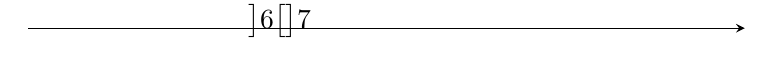
\begin{tikzpicture}[scale=0.7,>=stealth]
				 \draw[->](-4,0)->(9,0);
				 \def\skipInterval{0.5cm}
				\def\colorInterval{blue} 
				 \IntervalLR{6}{9}\IntervalGLF{\big]}{$6$}{}{}
				\IntervalLR{-4}{-2} 
				 \IntervalGRF{}{}{\big[}{-2}
				\IntervalLR{7}{9} 
				 \IntervalGRF{\big]}{$7$}{}{}
			\end{tikzpicture}
		 }
	} 
\end{ex}

% nguồn: MaHoaNH_TracNghiem_Lop10
\begin{ex}%[0D1B3-1]%[ma:274b637d]
	Cho các tập hợp $M=[-3;6]$  và $N=(-\infty; -2)\cup (3;+\infty)$. Khi đó $M\cap N$ là
	 \choice
		{$(-\infty;-2)\cup (3;6)$} 
		{$(-\infty;-2)\cup  [3;+\infty)$}
		{\True  $[-3;-2)\cup (3;6]$}
		 {$(-3;-2)\cup (3;6)$}
	 \loigiai{
		Biểu diễn  trục số:
		\begin{center}
			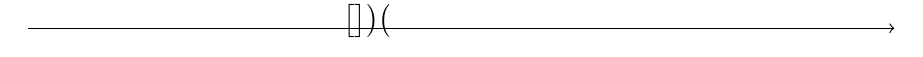
\begin{tikzpicture}
					\draw[->](-4,0)->(7,0); 
					\IntervalLR{-4}{-3} 
					 \IntervalGR{}{}{\big[}{-3}
					\IntervalLR{6}{6.9} 
					\IntervalGR{\big]}{6}{}{} 
					 \IntervalLR{-2}{3}
					\def\skipInterval{0.5cm} 
					\IntervalGLF{\big)}{-2}{\big (}{3} 
				\end{tikzpicture}
		\end{center}
		Từ  hình vẽ, ta có
	 Khi đó: $M\cap N= [-3;-2)\cup (3;6]$.}
\end{ex}

% nguồn: MaHoaNH_TracNghiem_Lop10
\begin{ex}%[0D1Y3-1]%[ma:ce1f4a38]
	 \immini[thm]
	 {
	 Cho $A,B$ là hai tập hợp bất kì. Phần gạch chéo trong hình vẽ bên là tập hợp nào sau đây?
	 \choice
		{$A \setminus  B$}
		{$B \setminus A$} 
		{\True  $A \cap B$}
		{$A \cup  B$}
		} 
		{ 
		\begin{tikzpicture}[scale=0.6]
				\draw (0,0) ellipse (2cm and  1cm);
				\draw (2,0) ellipse (1.5cm and 0.7cm); 
				\begin{scope}
					 \clip (0,0) ellipse (2cm and 1cm);
					\fill[pattern=north west lines] (2,0) ellipse (1.5cm  and 0.7cm);
				\end{scope}
				\node at (0,0) [above left] {$A$}; 
				\node at (2,0)  [right] {$B$};
			\end{tikzpicture}
		} 
	\loigiai{ 
		Phần gạch chéo trong hình minh họa cho các phần tử thuộc  cả tập $A$ và $B$.
	 }
\end{ex}

% nguồn: MaHoaNH_TracNghiem_Lop10
\begin{ex}%[0D1B3-1]%[ma:dacc29c2]
	Cho $A$, $B$ là hai tập  hợp bất kì. Phần tô màu trong hình vẽ bên dưới là tập hợp nào sau đây?\\
	\begin{center}
	\def\firstcircle{(0,0) circle (1.5cm)} 
	\def\secondcircle{(0:2cm) circle  (1.5cm)}
		\colorlet{circle  edge}{blue!50}
		\colorlet{circle  area}{blue!20}
		\tikzset{filled/.style={fill=circle  area, draw=circle edge, thick},
		outline/.style={draw=circle edge, thick}} 
		\setlength{\parskip}{5mm} 
		\begin{tikzpicture}
				\begin{scope}
					\clip \firstcircle; 
					 \fill[black] \secondcircle;
				\end{scope}
				\draw[outline]  \firstcircle node {$A$};
				\draw[outline] \secondcircle node  {$B$};
			\end{tikzpicture}
	\end{center}
	\choice 
		{$A\cup  B$}
		 {$B\setminus A$}
		{$A\setminus  B$}
		{\True  $A\cap B$}
	 \loigiai{
	Theo biểu đồ Ven thì phần gạch sọc  trong hình vẽ là tập hợp $A\cap B$.}
\end{ex}

% nguồn: MaHoaNH_TracNghiem_Lop10
\begin{ex}%[0D1B3-1]%[ma:8bce89f5]
	Cho tập hợp $A=(-\infty;3]$ và  $B=(1;+\infty)$. Tập hợp $A\cup B$ là
	 \choice
		{$(-\infty;1]$} 
		{$(-\infty;3]$} 
		{$(-\infty;1)\cup (1;3]$} 
		 {\True $(-\infty;+\infty)$}
	 \loigiai{
	\immini{ 
		\begin{tikzpicture}[xscale=0.7,thick,>=stealth']
				\draw[->](-3,0) node[left]{$A$}->(6,0); 
				 \IntervalLR{3}{6}
				 \IntervalGRF{]}{3}{}{}
			\end{tikzpicture}
		 \\
		\begin{tikzpicture}[xscale=0.7,thick,>=stealth']
				\draw[->](-3,0) node[left]{$B$}->(6,0); 
				 \IntervalLR{-3}{1}
				\IntervalGRF{}{}{(}{1} 
			\end{tikzpicture}
		 }
		 {
		\begin{tikzpicture}[xscale=0.7,thick,>=stealth']
				\draw[->](-3,0) node[left]{$A\cup B $}->(6,0); 
			\end{tikzpicture}
		} 
	 }
\end{ex}

% nguồn: MaHoaNH_TracNghiem_Lop10
\begin{ex}%[0D1B3-1]%[ma:f5230211]
	Cho tập hợp $A=(-\infty;4]$ và $B=(1;+\infty)$. Tập hợp $B\backslash A$  là
	\choice 
		{\True $(4;+\infty)$} 
		{$(-\infty;1)$} 
		 {$[1;+\infty)$}
		 {$[4;+\infty)$}
	 \loigiai{
	\immini{ 
		\begin{tikzpicture}[xscale=0.7,thick,>=stealth']
				 \draw[->](-2,0) node[left]{$A$}->(7,0);
				\IntervalLR{4}{7} 
				 \IntervalGRF{]}{4}{}{}
			\end{tikzpicture}
		 \\
		\begin{tikzpicture}[xscale=0.7,thick,>=stealth']
				\draw[->](-2,0) node[left]{$B$}->(7,0); 
				 \IntervalLR{-2}{1}
				\IntervalGRF{}{}{(}{1} 
			\end{tikzpicture}
		 }
		 {
		\begin{tikzpicture}[xscale=0.7,thick,>=stealth']
				\draw[->](-2,0) node[left]{$B\backslash  A$}->(7,0);
				 \IntervalLR{-2}{4}
				\IntervalGRF{}{}{(}{4} 
			\end{tikzpicture}
		} 
	 }
\end{ex}

% nguồn: MaHoaNH_TracNghiem_Lop10
\begin{ex}%[0D1B3-1]%[ma:7fa643c0]
	Cho hai tập hợp $A=(-3;3)$ và  $B=(0;+\infty)$. Tìm $A \cup B$.
	\choice 
		{$ A  \cup B = [-3;+\infty) $}
		 {$ A \cup B = (0;3) $}
		 {$ A \cup B = [-3;0) $}
		{\True $ A \cup B = (-3;+\infty) $} 
	\loigiai{ 
	\immini{Tập hợp $A=(-3;3)$ có biểu  diễn là}{
		\begin{tikzpicture}[scale=1,font=\footnotesize,line join = round,line cap = round,>=stealth]
				\draw[thick,->] (-2,0)  node[below=6pt]{$-\infty$} -- (0,0) node[scale=1.5]{\bf (} node[below=6pt]{$-3$} -- (3,0) node[scale=1.5]{\bf)} node[below=6pt]{$3$} -- (5,0) node[below=6pt]{$+\infty$};
				\foreach  \i in {1,...,10}
				\draw  ($(0,0)-(.2*\i,0)$) node[scale=.6]{/};
				 \draw ($(0,0)$) node[scale=.6]{/};
				\foreach \i in  {1,...,9}
				\draw ($(3,0)+(.2*\i,0)$) node[scale=.6]{/}; 
				 \draw ($(3,0)$) node[scale=.6]{/};
			\end{tikzpicture}
		 }
	\immini{Tập hợp $B=(0;+\infty)$ có biểu diễn  là}{
		\begin{tikzpicture}[scale=1,font=\footnotesize,line join = round,line cap = round,>=stealth]
				\draw[thick,->] (-2,0)  node[below=6pt]{$-\infty$}--(1,0) node[scale=1.5]{\bf (} node[below=6pt]{$0$}-- (5,0) node[below=6pt]{$+\infty$};
				\foreach \i in {1,...,15} 
				\draw  ($(1,0)-(.2*\i,0)$) node[scale=.6,rotate=60]{/};
				 \draw ($(1,0)$) node[scale=.6,rotate=60]{/};
			\end{tikzpicture}
		} 
		 \noindent Do đó $A \cup B=(-3;+\infty)$.
	} 
\end{ex}

% nguồn: MaHoaNH_TracNghiem_Lop10
\begin{ex}%[0D1K3-1]%[ma:ca8e50f4]
	Biểu diễn trên  trục số của tập hợp $\mathbb{R}\setminus \left(\left(-3;4\right) \cap \left[{0;2}\right)\right) $ là hình nào?
	 \def\dotEX{}
	 \choice
		 {
		\begin{tikzpicture}[xscale=0.5,thick,>=stealth']
				 \draw[->](-5,0)->(6,0);
				\IntervalLR{-5}{0} 
				\IntervalGRF{}{}{[}{0} 
				 \IntervalLR{2}{6}
				\IntervalGRF{)}{2}{}{} 
			\end{tikzpicture}
		 }
		{ 
		\begin{tikzpicture}[xscale=0.5,thick,>=stealth']
				 \draw[->](-5,0)->(6,0);
				 \IntervalLR{-5}{-3}
				\IntervalGRF{}{}{(}{-3} 
				 \IntervalLR{4}{6}
				\IntervalGRF{]}{4}{}{} 
			\end{tikzpicture}
		 }
		 {\True
		\begin{tikzpicture}[xscale=0.5,thick,>=stealth']
				\draw[->](-5,0)->(6,0); 
				\IntervalRF{)}{0}{[}{2} 
			\end{tikzpicture}
		} 
		 {
		\begin{tikzpicture}[xscale=0.5,thick,>=stealth']
				 \draw[->](-5,0)->(6,0);
				\IntervalRF{]}{-3}{[}{2} 
			\end{tikzpicture}
		 }
	 \loigiai{
		Ta có  $(-3;4)\cap [0;2)=[0;2)\Rightarrow$ $\mathbb{R}\setminus \left(\left(-3;4\right) \cap \left[{0;2}\right)\right)=(-\infty;0)\cap [2;+\infty)$ nên được biểu diễn trên trục số là
		\begin{center}
			\begin{tikzpicture}[xscale=0.5,thick,>=stealth']
					 \draw[->](-5,0)->(6,0);
					\IntervalRF{)}{0}{[}{2} 
				\end{tikzpicture}
		\end{center}
	} 
\end{ex}


%%%%%%%%%%%%%%%% ĐÚNG/SAI %%%%%%%%%%%%%%%%

% nguồn: MaHoaNH_DungSai_Lop10
\begin{ex}%[0D1N3-1]%[ma:3acfa869]
	 Cho các tập hợp $A=\{0;2;3;5\}$, $B=\{-1;2;4;5;6\}$, $C=\{-2;0;1;3;4\}$.
	\choiceTF 
		{\True $A\cap B=\{2;5\}$} 
		{$A\cup B=\{-1;0;2;3;5;6\}$} 
		{$B\cap C=\{2;3;4\}$} 
		{\True $B\cup  C=\{-2;-1;0;1;2;3;4;5;6\}$}
	 \loigiai{
		\begin{itemchoice}
			\itemch $A\cap B=\{2;5\}$. 
			\itemch $A\cup  B=\{-1;0;2;3;4;5;6\}$.
			\itemch  $B\cap C=\{4\}$.
			\itemch $B\cup  C=\{-2;-1;0;1;2;3;4;5;6\}$.
		\end{itemchoice}
	} 
\end{ex}

% nguồn: MaHoaNH_DungSai_Lop10
\begin{ex}%[0D1N3-1]%[ma:ec17cb53]
	Cho các tập hợp $A=\{x\in  \mathbb{N}|x<5\}$, $B=\{x\in\mathbb{Z}|x^2+x-2=0\}$ và $C=\{-2;-1;1;4\}$.
	 \choiceTF
		{ $A\cap B=\{-2;1\}$} 
		{\True  $A\cup B=\{-2;0;1;2;3;4\}$}
		 {$A\cup C=\{-2;-1;0;1;2;3;4;5\}$}
		 { $B\cap C=\{-2\}$}
	\loigiai{Ta có $A=\{0;1;2;3;4\}$, $B=\{-2;1\}$, $C=\{-2;-1;1;4\}$. 
		\begin{itemchoice}
			 \itemch $A\cap B=\{1\}$.
			\itemch $A\cup B=\{-2;0;1;2;3;4\}$. 
			\itemch $A\backslash  B=\{0;2;3;4\}$.
			\itemch  $B\backslash A=\{-2\}$.
		\end{itemchoice}
	} 
\end{ex}


%%%%%%%%%%%%%%%% TRẢ LỜI NGẮN %%%%%%%%%%%%%%%%

% nguồn: MaHoaNH_TraLoiNgan_Lop10
\begin{bt}%[0D1H3-1]%[ma:c37af74c]
	Một lớp học có 25 học sinh giỏi môn Toán, 23 học sinh giỏi môn Lý, 14 học sinh giỏi cả môn Toán và  Lý và có 6 học sinh không giỏi môn nào cả. Hỏi lớp đó có bao nhiêu học sinh?
	\shortans{40} 
	\loigiai{ 
		Gọi $\Omega, A, B$ lần lượt là tập hợp số  học sinh của cả lớp, tập hợp số học sinh giỏi Toán, tập hợp số học $\sinh$ giỏi Lý.\\
		Ta có $n(A)=25, n(B)=23,  n(A \cap B)=14$.\\
		 $n(A\cup B)=25+23-14=34$.\\
		 $n(\Omega)=34+6=40$.
	 }
\end{bt}

% nguồn: MaHoaNH_TraLoiNgan_Lop10
\begin{bt}%[0D1H3-1]%[ma:354bbbd6]
	Cho hai tập hợp khác rỗng $A=(m-1;8]$ và $B=(-10;2m+2)$,  $m\in\mathbb{R}$. Có bao nhiêu giá trị nguyên dương của tham số $m$ để $A\cap B\ne\varnothing$?
	\shortans{8} 
	\loigiai{ 
		Điều kiện  để $A, B$ khác rỗng $\heva{&m-1<8\\ &2m+2>-10}\Leftrightarrow\heva{&m<9\\ &m>-6}\Leftrightarrow-6<m<9$.\\
		Điều kiện để $A\cap  B\ne\varnothing$ là $m-1<2m+2\Leftrightarrow m>-3$.\\
		Kết hợp điều kiện  $-3<m<9$.\\
		Giá trị nguyên dương của $m$  là $1, 2, 3, 4, 5, 6, 7, 8$.\\
		Có 8 giá trị nguyên dương  thỏa mãn.
	} 
\end{bt}

% nguồn: MaHoaNH_TraLoiNgan_Lop10
\begin{bt}%[0D1V3-1]%[ma:2d7ab131]
	Cho các tập hợp $A=\left\{x\in \mathbb{Q}\mid  \left(x-1\right)\left(3x-2\right)\left(x+\sqrt{2} \right)=0\right\}$ và\break $B=\left\{x\in \mathbb{R}\mid \left(2+x\right)\left(3x-m^2+4\right)=0\right\}$. Tích các giá trị của tham số $m$ để $n\left(A\cup B\right)=3$ bằng bao nhiêu?
	\shortans{42} 
	\loigiai{ 
		Xét  các phương trình
		\[\left(x-1\right)\left(3x-2\right)\left(x+\sqrt{2} \right)=0\Leftrightarrow \left[\begin{array}{l}{x=1\in \mathbb{Q}} \\ {x=\dfrac{2}{3} \in \mathbb{Q}} \\ {x=-\sqrt{2} \notin \mathbb{Q}}
	\end{array}\right. \Rightarrow A=\left\{1; \dfrac{2}{3} \right\}.\]
	\[\left(2+x\right)\left(3x-m^2+4\right)=0\Leftrightarrow \hoac{&x=-2\\&x=\dfrac{m^2-4}{3}.} 
	 \]
	Ta thấy $m^2\ge 0$, $\forall m\in \mathbb{R}\Rightarrow \dfrac{m^2-4}{3} \ge-\dfrac{4}{3}$, $\forall m\in  \mathbb{R}\Rightarrow-2\ne \dfrac{m^2-4}{3}$ $\Rightarrow B=\left\{\dfrac{m^2-4}{3};-2\right\}$.\\
	Khi đó $n\left(A\cup B\right)=3$ $\Leftrightarrow \hoac{&\dfrac{m^2-4}{3}=1\\  &\dfrac{m^2-4}{3}=\dfrac{2}{3}} \Leftrightarrow \hoac{&m=\pm \sqrt{7}\\&m=\pm \sqrt{6}}$.\\
	Suy ra tích các giá  trị của tham số $m$ là $-\sqrt{7}\cdot \sqrt{7}\cdot \left(-\sqrt{6} \right)\cdot \sqrt{6}=42$.
 }
\end{bt}


%%%%%%%%%%%%%%%% TỰ LUẬN %%%%%%%%%%%%%%%%

% nguồn: MaHoaNH_TuLuan_Lop10
\begin{bt}%[0D1B3-1]%[ma:285b4da0]
	Cho $A=(-\infty;-2]$, $B=[3;+\infty)$, $C=(0;4)$.  Tìm $(A\cup B)\cap C$?
	\loigiai{Ta có: $A\cup  B=(-\infty;-2]\cup[3;+\infty)$.\\
	Vậy $(A\cup B)\cap  C=[3;4)$.}
\end{bt}

% nguồn: MaHoaNH_TuLuan_Lop10
\begin{bt}%[0D1K3-1]%[ma:d55a9fc9]
	 Cho tập $A=(-1;3]$ và $B=[m-2;m+3]$. Tìm $m$ để $A\cap B=\varnothing$.
	\loigiai{ 
	Ta có $A\cap  B=\varnothing$ khi
	\[\hoac{&m-2>3\\&m+3\le-1}\Leftrightarrow\hoac{&m>5\\&m\le-4.}\] 
	Vậy $m\le-4$ hoặc  $m>5$.
	 }
\end{bt}

% nguồn: MaHoaNH_TuLuan_Lop10
\begin{bt}%[0D1B3-1]%[ma:10860931]
	Cho các tập hợp: $ A=\{1,2,3,4,5,6,7,8,9\} $; $ B=\{1,2,3,4\} $; $C=\{2,4,6,8\}  $. Hãy xác định: $ C_AB, C_AC, C_A (B \cup C) $.
	 \loigiai{
		\begin{listEX}
			\item $C_AB  =\{5,6,7,8,9\}$.
			\item $C_AC=\{1,3,5,7,9\}  $.
			\item  $C_A(B\cup C)=\{5,7,9\} $.
		\end{listEX}
	 }
\end{bt}

% nguồn: MaHoaNH_TuLuan_Lop10
\begin{bt}%[0D1B3-1]%[0D1B3-2]%[ma:8a69eb7d]
	Cho hai tập hợp $A=[2;+\infty)$,  $B=(-1;5]$. Tìm: $A\cap B$, $A\cup B$, $A\setminus B$, $\mathrm{C}_\mathbb{R}^A$.
	 \loigiai{
		\begin{eqnarray*}
			&A\cap  B &=\left[2;5\right].\\
			 &A\cup B &=\left(1;+\infty\right).\\
			&A\setminus B  &=\left(5;+\infty\right).\\
			&\mathrm{C}_\mathbb{R}^A  &=\left(-\infty;2\right).
		\end{eqnarray*}
	} 
\end{bt}

% nguồn: MaHoaNH_TuLuan_Lop10
\begin{bt}%[0D1B3-1]%[0D1B3-2]%[ma:e90d04ba]
	Cho $3$ tập hợp  $A=[-1;3)$, $B=(-\infty;1)$, $C=(-1;1]$.\\
	Xác định các tập hợp: $A\cup B$,  $A\setminus B$, $\left(A\cap B\right)\setminus C$.
	\loigiai{ 
		\begin{itemize}
			 \item $A\cup B=(-\infty;3)$.
			 \item $A\setminus B=[1;3)$.
			\item $\left(A\cap B\right)=[-1;1)\Rightarrow \left(A\cap  B\right)\setminus C=\{-1\}$.
		\end{itemize}
	 }
\end{bt}

% nguồn: MaHoaNH_TuLuan_Lop10
\begin{bt}%[0D1K3-1]%[ma:1448439f]
	Xác định  các tập hợp $A$, $B$ sao cho:
	\begin{enumerate}
		 \item $A\cap B=\left\{{0,1,2,3,4}\right\}$; $A\setminus B=\left\{{-3,-2}\right\}$; $B\setminus A=\left\{{6,9,10}\right\}$.
		\item $A\cap B=\left\{{1,2,3}\right\}$; $A\setminus B=\left\{{4,5}\right\}$; $B\setminus  A=\left\{{6,9}\right\}$.
	\end{enumerate}
	 \loigiai{
		\begin{enumerate}
			\item  $A=\{-2;-3;0;1;2;3;4\}$, $B=\{0;1;2;3;4;6;9;10\}$.
			\item  $A=\{1;2;3;4;5\}$, $\{1;2;3;6;9\}$.
		\end{enumerate}
	} 
\end{bt}

% nguồn: MaHoaNH_TuLuan_Lop10
\begin{bt}%[0D1K3-1]%[ma:8ac335ca]
	Tìm tất cả các tập hợp $X$  sao cho:
	\begin{enumerate}
		\item $\left\{{1,2}\right\}\subset X\subset \left\{{1,2,3,4,5}\right\}$. 
		\item  $\left\{{1,2}\right\}\cup X=\left\{{1,2,3,4}\right\}$.
		\item $X\subset \left\{{1,2,3,4}\right\}$, $X\subset \left\{{0,2,4,6,8}\right\}$. 
	\end{enumerate}
	 \loigiai{
		\begin{enumerate}
			\item Các tập hợp $X$ thỏa  bao gồm: $\{1;2\}$, $\{1;2;3\}$, $\{1;2;4\}$, $\{1;2;5\}$, $\{1;2;3;4\}$, $\{1;2;3;5\}$, $\{1;2;4;5\}$, $\{1;2;3;4;5\}$.
			\item Các tập  hợp $X$ thỏa bao gồm: $\{3;4\}$, $\{1;3;4\}$, $\{2;3;4\}$, $\{1;2;3;4\}$.
			\item  Các tập hợp $X$ thỏa bao gồm: $\varnothing$, $\{2\}$, $\{4\}$, $\{2;4\}$.
		\end{enumerate}
	 }
\end{bt}

% nguồn: MaHoaNH_TuLuan_Lop10
\begin{bt}%[0D1K3-1]%[ma:be193707]
	Cho ba tập hợp $A=\{n\in\mathbb{N}\mid n\geq 2\}$, $B=\left\{x\in\mathbb{N}\mid (x-5)\left(x^2+1\right)<0\right\}$  và $C=\left\{k\in\mathbb{N}\mid dle| \dfrac{2k+12}{k^2+k} \text{là số nguyên}\right\}$. Tìm tập hợp $A\cap B\cap C$.
	\loigiai{ 
	Ta  có $A=\{2;3;4;\ldots\}$.\\
	Vì $x^2+1>0$  với mọi $x\in\mathbb{R}$ nên
	\[(x-5)\left(x^2+1\right)<0  \Leftrightarrow x-5<0 \Leftrightarrow x<5.\]
	Suy ra $B=\{0;1;2;3;4\}$.\\ 
	Vì vậy  $A\cap B=\{2;3;4\}$.\\
	Mặt khác, giả sử  $k\in A\cap B\cap C$ thì $k\in A$, $k\in B$ và $k\in C$. Do đó, ta thử $k=2$, $k=3$, $k=4$ vào biểu thức $\dfrac{2k+12}{k^2+k}$.
	\begin{itemize}
		\item Với $k=2$ ta được $\dfrac{2\cdot  2+12}{2^2+2} = \dfrac{8}{3}$ không nguyên.
		\item Với $k=3$ ta được $\dfrac{2\cdot 3+12}{3^2+3} = \dfrac{3}{2}$ không nguyên. 
		\item Với $k=4$ ta được  $\dfrac{2\cdot 4+12}{4^2+4} = 1$ nguyên.
	\end{itemize}
	Vậy $A\cap B\cap  C=\{4\}$.
	 }
\end{bt}

% nguồn: MaHoaNH_TuLuan_Lop10
\begin{bt}%[0D1B3-1]%[ma:e3215038]
	Cho $ A=\{1,2,3,4,5\} $ và $ B=\{1,3,5,7,9,11\} $. Hãy tìm 
	\begin{enumEX}{2}
		\item $ C=A  \cup B $.
		\item $ C=A\cap B $. 
		\item  $ C= (A\cup B) \setminus (A \cap B) $.
		 \item $ C=(a \setminus B) \cup (B \setminus A) $.
	\end{enumEX}
	 \loigiai{
		\begin{enumEX}{2}
			\item $ C=\{1,2,3,4,5,7,9,11\} $. 
			\item $  C=\{1,3,5\} $.
			\item  $ C=\{2,4,7,9,11\} $.
			\item  $ C=\{2,4,7,9,11\} $.
		\end{enumEX}
	} 
\end{bt}

% nguồn: MaHoaNH_TuLuan_Lop10
\begin{bt}%[0D1B3-1]%[0D1B3-2]%[ma:d9ffc59e]
	Cho các tập hợp\\ 
	$A=\{-3;5;6\}$; $B=\{x\in\mathbb{R}\colon x^2-4x-5=0\}$; 
	 $C=\{x\in\mathbb{N}\colon(x-2)(x^2+5x-6)=0\}$.
	\begin{listEX}[1]
		\item Viết tập hợp $B$  và $C$ dưới dạng liệt kê các phần tử. Tìm $A\cap B$; $A\cup C$.
		\item Tìm $(A\cup  B)\setminus C$; $(A\setminus B)\cap C$.
	\end{listEX}
	\loigiai{ 
		\begin{itemize}
			\item Ta có 
			\begin{itemize}
				\item $x^2-4x-5=0\Leftrightarrow \hoac{&x=-1\\&x=5}$.  Do đó $B=\{-1;5\}$.
				\item  $(x-2)(x^2+5x-6)=0\Leftrightarrow \hoac{&x=2\in\mathbb{N}\\&x=1\in\mathbb{N}\\&x=-6\notin\mathbb{N}}$. Do đó $C=\{1;2\}$.
			\end{itemize}
			Từ đó ta có  $A\cap B=\{5\}$; $A\cup C=\{-3;1;2;5;6\}$.
			\item 
			\begin{itemize}
				\item Ta có $A\cup B=\{-3;  -1; 5; 6\}$ nên $(A\cup B)\setminus C=\{-3; -1; 5; 6\}$.
				\item Ta có $A\setminus B=\{-3;  6\}$ nên $(A\setminus B)\cap C=\varnothing$.
			\end{itemize}
	\end{itemize}}
\end{bt}

% nguồn: MaHoaNH_TuLuan_Lop10
\begin{bt}%[0D1B3-1]%[0D1B3-2]%[ma:0767f13d]
	Cho các tập hợp\\ 
	 $A=\{-1;3;5\}$; $B=\{x\in\mathbb{R}\colon x^2-6x+5=0\}$;
	 $C=\{x\in\mathbb{N}\colon(x-3)(x^2+5x-6)=0\}$.
	\begin{listEX}[1]
		 \item Viết tập hợp $B$ và $C$ dưới dạng liệt kê các phần tử. Tìm $A\cap B$; $A\cup C$.
		\item Tìm $(A\cup B)\setminus C$; $(A\setminus B)\cap C$. 
	\end{listEX}
	\loigiai{ 
		\begin{listEX}
			 \item Ta có
			\begin{itemize}
				\item $x^2-6x+5=0\Leftrightarrow \hoac{&x=1\\&x=5}$. Do đó $B=\{1;5\}$. 
				\item  $(x-3)(x^2+5x-6)=0\Leftrightarrow \hoac{&x=3\in\mathbb{N}\\&x=1\in\mathbb{N}\\&x=-6\notin\mathbb{N}}$. Do đó $C=\{1;3\}$.
			\end{itemize}
			 Từ đó ta có $A\cap B=\{5\}$; $A\cup C=\{-1;1;3;5\}$.
			 \item
			\begin{itemize}
				\item Ta có $A\cup B=\{-1; 1; 3; 5\}$ nên $(A\cup B)\setminus C=\{-1; 5\}$. 
				\item Ta có $A\setminus  B=\{-1; 3\}$ nên $A\setminus B)\cap C=\{3\}$.
			\end{itemize}
	\end{listEX}}
\end{bt}

% nguồn: MaHoaNH_TuLuan_Lop10
\begin{bt}%[0D1K3-1]%[ma:b5dfb9a4]
	 Tìm $A\cap B;A\setminus B;B\setminus A$ với:
	\begin{enumerate}
		\item $A=\left\{{2,4,7,8,9,12}\right\}$;  $B=\left\{{2,8,9,12}\right\}$.
		\item $A=\left\{{2,4,6,9}\right\}$;  $B=\left\{{1,2,3,4}\right\}$.
		\item $A=\left\{{x\in  \mathbb{R}\left|{2x^2-3x+1=0}\right.}\right\}$; $B=\left\{{x\in \mathbb{R}\left|{\left|{2x-1}\right|=1}\right.}\right\}$.
		\item $A=$ Tập các ước số của $12$; $B=$ Tập các ước số của  $18$.
		\item $A=\left\{{x\in \mathbb{R}\left|{(x+1)\left(x-2\right)\left(x^2-8x+15\right)=0}\right.}\right\}$; $B=$ Tập  các số nguyên tố có một chữ số.
		\item $A=\left\{{x\in \mathbb{Z}\left|{x^2<4}\right.}\right\}$; $B=\left\{{x\in \mathbb{Z}\left|{\left(5x-3x^2\right)\left(x^2-2x-3\right)=0}\right.}\right\}$. 
		\item  $A=\left\{{x\in \mathbb{N}\left|{\left(x^2-9\right)\left(x^2-5x-6\right)=0}\right.}\right\}$; $B=\left\{x\in \mathbb{N}|x\text{là số nguyên tố,}x\le 5\right\}$.
	\end{enumerate}
	 \loigiai{
		\begin{enumerate}
			\item  $A\cap B=\{2;8;9;12\}$, $A\setminus B=\{4;7\}$, $B\setminus A=\varnothing$.
			\item $A\cap B=\{2;4\}$, $A\setminus B=\{6;9\}$, $B\setminus  A=\{1;3\}$
			\item $A=\left\{\dfrac{1}{2};1\right\}$, $B=\{1;0\}$, $A\cap B=\{1\}$, $A\setminus  B=\left\{\dfrac{1}{2}\right\}$, $B\setminus A=\{0\}$
			\item $A=\{1;2;3;4;6;12\}$, $B=\{1;2;3;6;9;18\}$,  $A\cap B=\{1;2;3;6\}$, $A\setminus B=\{4;12\}$, $B\setminus A=\{9;18\}$
			\item $A=\{-1;2;3;5\}$, $B=\{2;3;5;7\}$, $A\cap B=\{2;3;5\}$, $A\setminus B=\{-1\}$,  $B\setminus A=\{7\}$
			 \item $A=\{-2;-1;0;1;2\}$, $B=\{0;-1;3\}$, $A\cap B=\{-1;0\}$, $A\setminus B=\{-2;1;2\}$, $B\setminus A=\{3\}$
			\item $A=\{3;6\}$, $B=\{2;3;5\}$, $A\cap  B=\{3\}$, $A\setminus B=\{6\}$, $B\setminus A=\{2;5\}$
		\end{enumerate}
	 }
\end{bt}

% nguồn: MaHoaNH_TuLuan_Lop10
\begin{bt}%[0D1K3-1]%[ma:0cd8cd11]
	Cho hai tập hợp $A$  và $B$. Biết tập hợp $B$ khác rỗng, số phần tử của tập $B$ gấp đôi số phần tử của tập $A\cap B$ và $A\cup B$ có $10$ phần tử. Hỏi tập $A$ và $B$ có bao nhiêu phần tử. Hãy xét các trường hợp xảy ra và dùng biểu đồ Ven minh họa.
	\loigiai{ 
		Gọi số phần tử của tập hợp $B$ là $2b$. Do số phần tử của $B$ gấp đôi số phần tử của $A\cap B$ nên $A\cap B$ có  $b$ phần tử.\\
		Vì $B$  khác rỗng và $A\cup B$ có $10$ phần tử nên $0<2b$ và $2b<10$ (nếu $2b=10$ thì $A=\varnothing\Rightarrow A\cap B=\varnothing$, suy ra $B=\varnothing$ (mâu thuẫn)).
	\immini{ 
		Từ  đó suy ra $0<b<5$. Ta xét các trường hợp sau:
		\begin{enumerate}
			\item $b=1$. Khi đó $B$ có $2$ phần tử và $A$ có $8$  phần tử;
			\item $b=2$. Khi  đó $B$ có $4$ phần tử và $A$ có $6$ phần tử;
			\item $b=3$. Khi đó $B$ có $6$ phần tử  và $A$ có $4$ phần tử;
			\item $b=4$. Khi đó $B$ có $8$ phần tử và $A$ có  $2$ phần tử.
		\end{enumerate}
		 }{
		\begin{tikzpicture}[pattern=north east lines]
				\scope 
				\clip (-2,-2) rectangle (2,2) 
					(1,0)  circle (1);
				 \fill (0,0) circle (1);
			\endscope
			 \scope
			 \clip (-2,-2) rectangle (2,2)
				(0,0) circle  (1);
			\fill (1,0) circle (1); 
		\endscope
		\draw (0,0) circle (1) 
			(0,1) node  [text=black,above] {$A$}
			(1,0) circle  (1)
			(1,1) node [text=black,above]  {$B$}
			(-2,-2) rectangle (3,2); 
		\end{tikzpicture}
		 }
	 }
\end{bt}
